%%%%%%%%%%%%%%%%%%%% author.tex %%%%%%%%%%%%%%%%%%%%%%%%%%%%%%%%%%%
%
% sample root file for your "contribution" to a contributed volume
%
% Use this file as a template for your own input.
%
%%%%%%%%%%%%%%%% Springer %%%%%%%%%%%%%%%%%%%%%%%%%%%%%%%%%%


% RECOMMENDED %%%%%%%%%%%%%%%%%%%%%%%%%%%%%%%%%%%%%%%%%%%%%%%%%%%
\documentclass[graybox]{svmult}

% choose options for [] as required from the list
% in the Reference Guide

\usepackage{mathptmx}       % selects Times Roman as basic font
\usepackage{helvet}         % selects Helvetica as sans-serif font
\usepackage{courier}        % selects Courier as typewriter font
\usepackage{type1cm}        % activate if the above 3 fonts are
                            % not available on your system
%
\usepackage{makeidx}         % allows index generation
\usepackage{graphicx}        % standard LaTeX graphics tool
                             % when including figure files
\usepackage{multicol}        % used for the two-column index
\usepackage[bottom]{footmisc}% places footnotes at page bottom

\usepackage[numbers]{natbib}
\usepackage{subfigure}
\newcommand{\stnote}[1]{\textcolor{blue}{\textbf{ST: #1}}}
\newcommand{\jgonote}[1]{\textcolor{green}{\textbf{JGO: #1}}}


% see the list of further useful packages
% in the Reference Guide

\makeindex             % used for the subject index
                       % please use the style svind.ist with
                       % your makeindex program

%%%%%%%%%%%%%%%%%%%%%%%%%%%%%%%%%%%%%%%%%%%%%%%%%%%%%%%%%%%%%%%%%%%%%%%%%%%%%%%%%%%%%%%%%

\begin{document}

\title*{Autonomously Acquiring Instance-Based Object Models}
% Use \titlerunning{Short Title} for an abbreviated version of
% your contribution title if the original one is too long
\author{John Oberlin and Stefanie Tellex}
% Use \authorrunning{Short Title} for an abbreviated version of
% your contribution title if the original one is too long
\institute{Brown University}
%
% Use the package "url.sty" to avoid
% problems with special characters
% used in your e-mail or web address
%
\maketitle

\abstract{A key aim of current research is to create robots that can reliably
manipulate generic objects.  However, in many applications,
general-purpose object detection or manipulation is not required: the
robot would be useful if it could recognize, localize, and manipulate
the relatively small set of specific objects most important in that
application, but do so with very high reliability.  The contribution
of this paper is to automate this adaptation process by formalizing a
grasping system as a hierarchy of bandit problems, enabling the robot
to apply learning techniques to adapt itself to manipulate specific
objects with increased accuracy.  The robot performs best arm
identification using a variant of Hoeffding races, enabling it to
quickly find an optimal arm and then move on to the next object.  Our
approach also incorporates knowledge from a prior defined in terms of
an ordering on the arms.  We demonstrate that our bandit-based
adaptation step significantly improves accuracy over a non-adaptive
system, enabling a robot to quickly and autonomously acquire models
for objects, and adaptively improve them through experience.
}


\section{Introduction}

.  Instance-based approaches that focus on
specific instances of objects can have higher accuracy but require
training by a human operator, which is time consuming and can be
difficult for a non-expert to perform~\citep{ork14, lai11, lai11a}.
Existing approaches to autonomously learn 3D object models still
require expensive ICP-based methods to localize objects, which are
susceptible to local minima and take time to
converge~\citep{krainin11}.


We present an approach that captures the high accuracy of
instance-based methods without the need for manually acquiring
training data by enabling a robot to learn to identify and grasp on a
per object basis. Our grasping and perception pipeline uses standard
computer vision techniques to perform data collection, feature
extraction, and training, along with active visual servoing for
localization.  This framework succeeds to some degree with many
objects, but reaches performance ceilings for specific objects for a
variety of reasons.



\section{Grasping Pipeline}


\section{Grasping System}

We first describe our instance-based object detection and pose
estimation pipeline, which uses standard computer vision algorithms
combined to achieve a simple software architecture, a high frame rate,
and high accuracy at recognition and pose
estimation. Section~\ref{sec:training} describes our approach to
enabling a robot to autonomously collect the data needed to perform
grasping with this pipeline.

Our recognition pipeline takes video from the robot, proposes a small
number of candidate object bounding boxes in each frame, and
classifies each candidate bounding box as belonging to a previously
encountered object class. Our object classes consist of object
instances rather than pure object categories.  Using instance
recognition means we cannot reliably detect categories, such as
``mugs,'' but the system will be able to detect, localize, and grasp
the specific instances for which it has models with much higher speed
and accuracy.  A visualization of data flow in the pipeline appears in
Figure~\ref{fig:system}.  \jgonote{This doesn't quite seem current:}
For each module, we formalize its input,
output, and reward function; each component can have multiple
implementations which better for different objects.  The following
sections describe how we can use this pipeline to learn which
implementation to use for specific objects; this learning dramatically
speeds up performance.

%% \begin{figure}
%% 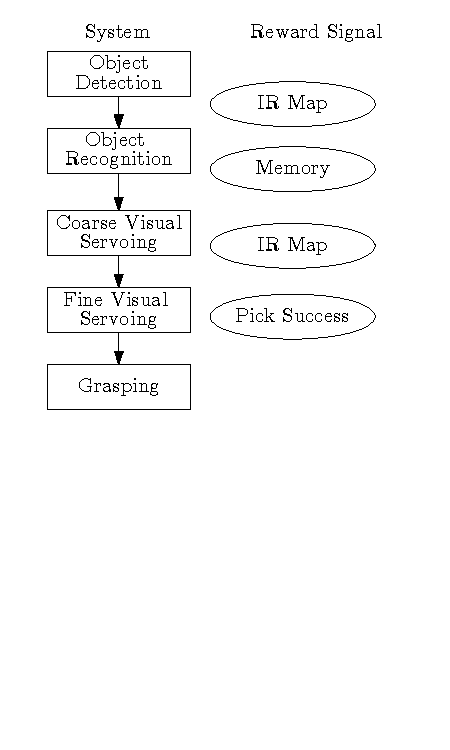
\includegraphics{system.pdf}
%% \caption{Data flow in our grasping system.\label{fig:system}}
%% \end{figure}

\subsection{Object Detection}
\label{sec:detection}

The input of the object detection component is an image, $I$; the
output is a set of candidate bounding boxes, $B$.  For object
detection we use a modified Canny algorithm which terminates before
the usual non-maximal suppression step~\citep{canny86}.

%\subsubsection{Detecting Objects Using Image Gradients}

We start by converting $I$ to YCbCr opponent color representation.
Then we apply $5 \times 5$ Sobel derivative filters~\citep{sobel95} to
each of the three channels and keep the square gradient magnitude. We
take a convex combination of the three channels, where Cb and Cr and
weighted the same and more heavily than Y.  After this we downsample,
apply the two Canny thresholds, and find connected components.  If a
connected component is contained in another, we discared the contained
component.  We throw out boxes which do not contain enough visual data
to classify.  We generate a candidate bounding box for each remaining
component by taking the smallest box which contains the component.

\subsection{Object Classification}
\label{sec:recognition}

The object recognition module takes as input a bounding box, $B$, and
outputs a label for that object, $c$, based on the robot's memory.
This label is used to identify the object and look up other
information about the object for grasping further down the pipeline.

For each object $c$ we wish to classify, we gather a set of example
crops $E_c$ which are candidate bounding boxes (derived as above)
which contain $c$. We extract dense SIFT features ~\citep{lowe99} from
all boxes of all classes and use k-means to extract a visual
vocabulary of SIFT features ~\citep{szeliski10}. We then construct a
Bag of Words feature vector for each image and augment it with a histogram of
colors which appear in that image.  The augmented feature vector is
incorporated into a k-nearest-neighbors model which we use to classify
objects at inference~\citep{szeliski10}. We use kNN because our
automated training process allows us to acquire as much high-quality
data as necessary to make the model work well, and kNN supports direct
matching to this large dataset.  

%% \jgonote{I would be careful to think about what "performing well" means to
%% us versus what it means to line2D, because I'm betting they use more objects.}
%% Existing approaches for
%% instance-based grasping such as LINE-2D require the order of $2000$ examples
%% whereas our SIFT-based approach performs well with only $200$
%% ~\citep{hinterstoisser12}.


%% The use of SIFT features is motivated by the instance level nature of
%% our task. State-of-the-art vision methods typically use
%% HOG~\citep{dalal05} features, but that choice is motivated by category
%% level recognition. \stnote{What about category level recognition
%%   motivates HOG or CNN?  Can you be more specific?}


%% is easy to rebuild online, which is a key
%% property a classifier should enjoy if it is to interact with our
%% framework in real time. State-of-the-art computer vision classifiers
%% currently employ SVM's ~\citep{} or other models which require
%% expensive training. Using such a model would introduce a training step
%% in the inside loop of our data collection process, which would be
%% costly in either engineering or time.  It is possible to use kNN
%% during the online collection process and then train a stronger
%% classifier in the background at higher latency, essentially
%% introducing a cascading step in the data collection process.

\begin{figure*}
\subfigure[Raw image from the camera.]{
  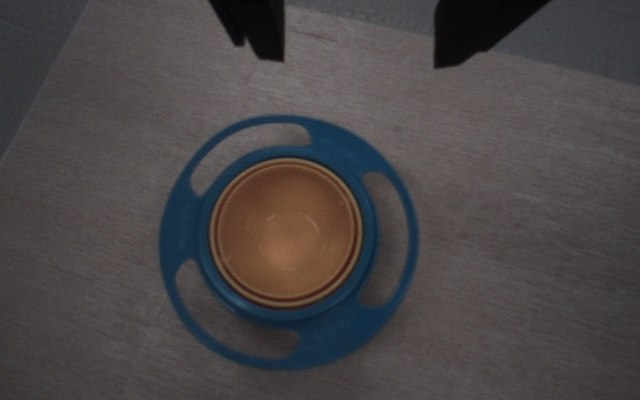
\includegraphics[width=0.25\linewidth]{figures/objectness_raw.png}}%
\subfigure[Candidate bounding boxes.\label{fig:segment}]{
  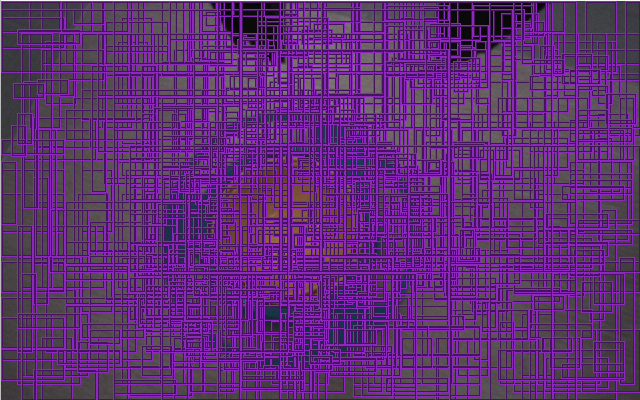
\includegraphics[width=0.25\linewidth]{figures/objectness_purple.png}}%
\subfigure[Integral image objectness map.\label{fig:objectness}]{
  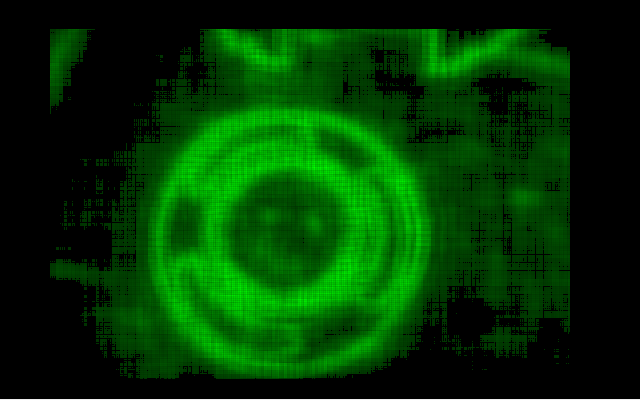
\includegraphics[width=0.25\linewidth]{figures/objectness_map.png}}%
\subfigure[Candidate bounding boxes.\label{fig:bounding_boxes}]{
  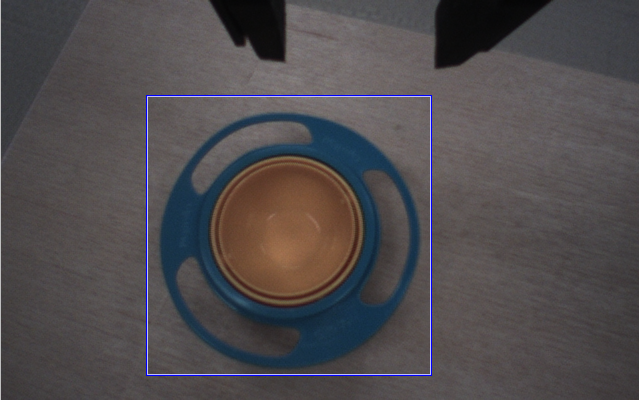
\includegraphics[width=0.25\linewidth]{figures/objectness_boxes1.png}}
\caption{The object detection pipeline, showing a raw image from the
  camera, the integral image computed using objectness, and candidate
  bounding boxes.\label{fig:object_detection}}
\end{figure*}



 
\subsection{Pose Estimation}

We use the image gradient for object detection and pose estimation. During
object detection, the gradient of the whole image is the first step in the Canny pipeline.
For pose estimation,  we require a crop of  image gradient of the object
at a specific, known pose. 

%We denote the gradient by
%\begin{align}
%\Delta I = \left( \frac{\partial I}{\partial x}, \frac{\partial I}{\partial y} \right)
%\end{align}

As in bounding box proposal, we approximate the gradient using 
$5 \times 5$ Sobel derivative filters~\citep{sobel95}, but we use a
different convex combination of the channels which focuses even less
on the Y channel.  Camera noise in the color channels is significant. To
cope with the noise, we marginalize the gradient estimate over several
frames taken from the same location, providing a much cleaner signal which matches more robustly.  To estimate 
pose, we rotate our training image and find the closest match to the 
image currently recorded from the camera, as detected and localized via 
the pipeline in Section~\ref{sec:detection} and~\ref{sec:recognition}.

In order to match our template image with the crop observed at pick time,
we remove the mean from and $L^2$ normalize the template and the crop.
Removing the mean provides invariance to bias, and normalizing introduces
invariance to scaling, which both help account somewhat
for lighting. 

\subsection{Identifying Grasp Points}

To identify a grasp points, we combine a depth map of the object with
a model of the gripper.  The depth map appears in
Figure~\ref{fig:depth_map} and is acquired by moving the rangefinder
on the arm through a raster scan over the object.  The grasp model
scores each potential grasp according to a linear model of the gripper
to estimate grasp success. A default algorithm picks the
highest-scoring grasp point using hand designed linear filters, but
frequently this point is not actually a good grasp, because the object
might slip out of the robot's gripper or part of the object may not be
visible in IR.  The input to this module is the 3d pose of the object,
and the output is a grasp point $(x, y, \theta)$; at this point we
assume only crane grasps rather than full 3d grasping, where $\theta$
is the angle which the gripper assumes for the grasp.



\subsection{Closed-Loop Grasping}

To grasp an object, we first scan the work area by moving the camera
until the object is detected and recognized.  Then we perform active
visual servoing to move the arm directly above the object.  Next, we
perform orientation servoing using the pose estimation
algorithm. Because these components are instance-based, they report
position and orientation with high accuracy, enabling us to use a
proportional controller (with no derivative or integral terms) to move
the arm into position.





\subsection{Autonomous Training}
\label{sec:training}

An object model in our framework consists of the following elements:
\begin{itemize}
\item cropped object templates (roughly 200), $t^1 ... t^K$
\item depth map, $D$, which consists of a point cloud, $(x, y, z, r, g, b)$.
\item cropped gradient template, $t_0$
\end{itemize}

To train our model, the robot first moves the object to a known pose,
then acquires images that are annotated with a pose as well as a
cropped bounding box for training.  Once the object has been moved to
a known pose, we acquire the object model by moving the camera around
the object, extracting bounding boxes from the resulting imgages, and
storing the resulting crops.


%% \begin{figure}
%%   \textbf{GraspObject()}
%%   \begin{algorithmic}
%%     \WHILE {true}
%%       \STATE $I \gets loadImage()$
%%       \STATE $B \gets Attempt a grasp.$
%%       \IF {grasp is successful}
%%         \STATE Move object to training area.
%%         \STATE Map(object).
%%       \ENDIF
%%     \ENDWHILE
%%   \end{algorithmic}
%%   \caption{The high-level object-learning algorithm.\label{alg:learning}}
%% \end{figure}


%% \begin{figure}
%%   \textbf{Map}
%%   \begin{algorithmic}
%%     \FOR {$(x^k, y^k, z^k) \in scan$}
%%     \STATE $I^k \gets ImageAt (x^k, y^k, z^k)$
%%     \STATE $t^k \gets Crop(I^k)$ using the approach described in Section~\ref{sec:detection}
%%     \STATE $D^k \gets PointAt(x^k, y^k, z^k)$
%%     \ENDFOR
%%   \end{algorithmic}
%%   \caption{The high-level algorithm for acquiring visual and grasping
%%     models of objects.}
%% \end{figure}


\citet{tellex11}


\bibliographystyle{plainnat}
\bibliography{main}

\end{document}
